\documentclass[dvipsnames]{article}
\usepackage{marvosym}

%...TikZ & PGF
\usepackage{pgfplots}
\pgfplotsset{compat=1.11}
\tikzset{>=latex}
\usetikzlibrary{calc,math}
\usepackage{tikzsymbols}
\usepgfplotslibrary{fillbetween}
\usetikzlibrary{decorations.markings} 
\usetikzlibrary{arrows.meta} %...APP2 for arrows as objects and images
\usetikzlibrary{backgrounds} %...For shading portions of graphs
\usetikzlibrary{patterns} %...Unit 5 Problems
\usetikzlibrary{shapes.geometric} %...For drawing cylinders in Unit 2
\tikzset{
    mark position/.style args={#1(#2)}{
        postaction={
            decorate,
            decoration={
                markings,
                mark=at position #1 with \coordinate (#2);
            }
        }
    }
} %...See https://tex.stackexchange.com/questions/43960/define-node-at-relative-coordinates-of-draw-plot

\tikzset{
    declare function = {trajectoryequation10(\x,\vi,\thetai)= tan(\thetai)*\x - 10*\x^2/(2*(\vi*cos(\thetai))^2);},
    declare function = {trajectoryequation(\x,\vi,\thetai)= tan(\thetai)*\x - 9.8*\x^2/(2*(\vi*cos(\thetai))^2);},
    declare function = {patheq(\x,\yi,\vi,\thetai)= \yi + tan(\thetai)*\x - 9.8*\x^2/(2*(\vi*cos(\thetai))^2);},
    declare function = {patheqten(\x,\yi,\vi,\thetai)= \yi + tan(\thetai)*\x - 10*\x^2/(2*(\vi*cos(\thetai))^2);} %like patheq but with gravity = 10
}

%...siunitx
\usepackage{siunitx}
\DeclareSIUnit{\nothing}{\relax}
\def\mymu{\SI{}{\micro\nothing} }
\DeclareSIUnit\mmHg{mmHg}
\DeclareSIUnit{\mile}{mi}
%...NOTE: "The product symbol between the number and unit is set using the quantity-product option."

%...Other
\usepackage{amsthm}
\usepackage{amsmath}
\usepackage{amssymb}
\usepackage{cancel}
\usepackage{subcaption}
\usepackage{dashrule}
\usepackage{enumitem}
\usepackage{fontawesome}
\usepackage{multicol}
\usepackage{glossaries}
%\numberwithin{equation}{section}
\numberwithin{figure}{section}
\usepackage{float}
\usepackage{twemojis} %...twitter emojis
\usepackage{utfsym}
\newcommand{\R}{\mathbb{R}} %...real number symbol
\usepackage{graphicx}
\graphicspath{ {../Figures/} }
\usepackage{hyperref}
\hypersetup{colorlinks=true,
    linkcolor=blue,
    filecolor=magenta,
    urlcolor=cyan,}
\urlstyle{same}
\newcommand{\hdashline}{{\hdashrule{\textwidth}{0.5pt}{0.8mm}}}
\newcommand{\hgraydashline}{{\color{lightgray} \hdashrule{0.99\textwidth}{1pt}{0.8mm}}}

%...Miscellaneous user-defined symbols
\newcommand{\fnet}{F_{\text{net}}} %...For net force
\newcommand{\bvec}[1]{\vec{\mathbf{#1}}} %...bold vector
\newcommand{\bhat}[1]{\,\hat{\mathbf{#1}}} %...bold hat vector
\newcommand{\que}{\mathord{?}}  %...Question mark symbol in equation env
%...Define thick horizontal rule for examples:
\newcommand{\hhrule}{\hrule\hrule}
\let\oldtexttt\texttt% Store \texttt
\renewcommand{\texttt}[2][black]{\textcolor{#1}{\ttfamily #2}}% 

%...For use in the exam document class
\newif\ifprintmetasolutions


%...Decreases space above and below align and gather enironment
\makeatletter
\g@addto@macro\normalsize{%
  \setlength\abovedisplayskip{-3pt}
  \setlength\belowdisplayskip{6pt} 
}
\makeatother





\usepackage[margin=1in]{geometry}
\usepackage{OutilsGeomTikz}

%...Theorem for examples
\theoremstyle{definition}
\newtheorem{example}{Example}

%...Define colors for use in Unit 11: SHM and Waves
\pgfdeclarehorizontalshading{visiblelight}{50bp}{
color(0.00000000000000bp)=(red);
color(8.33333333333333bp)=(orange);
color(16.66666666666670bp)=(yellow);
color(25.00000000000000bp)=(green);
color(33.33333333333330bp)=(cyan);
color(41.66666666666670bp)=(blue);
color(50.00000000000000bp)=(violet)
}

\setlength\parindent{0pt}
\setlength{\parskip}{6pt}

\renewcommand{\thesubsubsection}{\thesubsection\alph{subsubsection}}
\begin{document}

\pagestyle{empty}

\begin{center}
    \resizebox{\linewidth}{!}{Physics}
\end{center}

\vspace{1cm}


\begin{center}
\resizebox{0.5\linewidth}{!}{
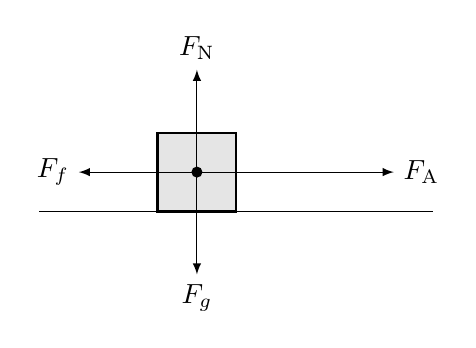
\begin{tikzpicture}
    \draw (0,0) -- (5,0);
    \draw[thick,fill=black!10] (1.5,0) rectangle ++(1,1);
    \fill (2,0.5) circle (2pt);
    \draw[->] (2,0.5) -- ++(0,+1.3) node[above] {$F_\mathrm{N}$};
    \draw[->] (2,0.5) -- ++(0,-1.3) node[below] {$F_g$};
    \draw[->] (2,0.5) -- ++(+2.5,0) node[right] {$F_\mathrm{A}$};
    \draw[->] (2,0.5) -- ++(-1.5,0) node[left] {$F_f$};
\end{tikzpicture}
}

\vspace{1cm}

\begin{tikzpicture}[declare function={t(\x)=\x/(18*cos(45));}]
    \begin{axis}[width=16cm,,height=10cm,
        axis lines=none,
        ylabel={$y$ (m)},
        xlabel={$x$ (m)},
        ymin=0,ymax=20,
        xmin=0,xmax=45,
        ytick={0,2,...,20},
        xtick={0,5,...,45},
        minor x tick num=1,
        grid=both,
        clip=false,
    ]
    \addplot[domain=0:40,red,thick] {trajectoryequation(x,18,45)+10};
    \def\myscale{0.3}
    \pgfplotsinvokeforeach{0,5,10,21,26,31,36,40}{
            \draw[fill=black] (#1,{trajectoryequation(#1,18,45)+10}) circle (2pt);
            \draw[dashed,->] (#1,{trajectoryequation(#1,18,45)+10}) -- ++(0,{\myscale*(18*sin(45) - 9.8*t(#1))});
            \draw[dashed,->] (#1,{trajectoryequation(#1,18,45)+10}) -- ++({\myscale*18*cos(45)},0);
            \draw[thick,->] (#1,{trajectoryequation(#1,18,45)+10}) -- ++({\myscale*18*cos(45)},{0.3*(18*sin(45) - 9.8*t(#1))});
            }
            
    %...For the apex:
    \draw[fill=black] (16.51,{trajectoryequation(16.51,18,45)+10}) circle (2pt);
    \draw[thick,->] (16.51,{trajectoryequation(16.51,18,45)+10}) -- ++({\myscale*18*cos(45)},0);

    %...For the initial point:
    \draw (0,{trajectoryequation(0,18,45)+10}) ++ (0,{\myscale*(18*sin(45))}) node[above] {$v_{iy}$};
    \draw (0,{trajectoryequation(0,18,45)+10}) ++ ({\myscale*(18*cos(45))},0) node[right] {$v_{ix}$};
    \draw (0,{trajectoryequation(0,18,45)+10}) ++ ({\myscale*(18*cos(45))},{\myscale*(18*sin(45))}) node[above left] {$v_i$};
    \end{axis}
\end{tikzpicture}
\end{center}

\end{document}
